\documentclass{article}
\usepackage[]{url}
\usepackage{graphicx}
\usepackage{hyperref}
\usepackage{mathtools}
\usepackage{tikz}
\usepackage{subcaption}

\begin{document}
\title{Collective motion of squirmers in confined environments}
\author{Roth Robin\\
\\
Supervisors: Van Landeghem Céline, Giraldi Laetitia,\\ Agathe Chouippe}
\date{May, 2024}
\maketitle

\tableofcontents

\section{Introduction}
This internship is the continuation of a project realised during the year. The main goal of the project was
to develop numerical methods for driving micro-robots composed of magnetic heads and flexible tails imitating spermatozoa, reffered to as squirmers.\\
A python code has been implemented during the project, it simulates the behaviors of two interacting squirmers by computing 
the forces and torques present.\\
\section{Context}
The collective behavior of active particles is well studied in the literature. 
The Vicsek model is frequently used to model these active particles. 
The aim of this internship is to perform a similar study considering squirmers, 
in various confined domains and to compare the collective motion of the squirmers with that of the active particles using the Vicsek model. 
The motion of the squirmers is simulated using two different models: a continuous model that approximates hydrodynamic and 
steric forces, and a full model using the finite element library Feel++.

\section{Objectives}
The main goal is to model the dynamics of a schoal of squirmers within confined environments, 

\section{Vicsek}
\subsection{Model}
\begin{center}
    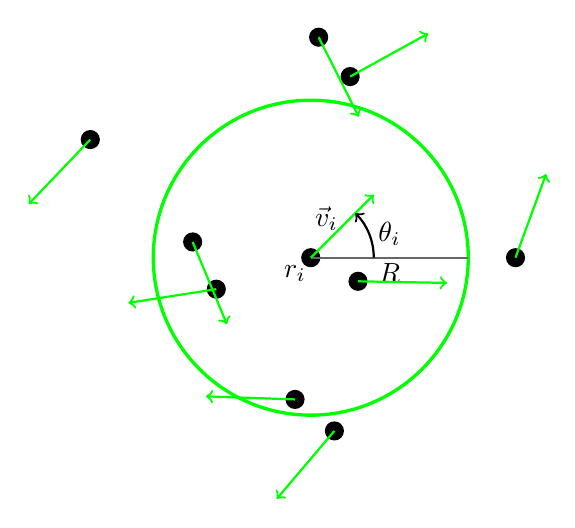
\begin{tikzpicture}
        \draw[color=green, very thick](0,0) circle (2);
        \node at (-0.2,-0.2) {{$r_i$}};
        \filldraw[color=black, fill=black, very thick](0,0) circle(0.1);
        \filldraw[color=black, fill=black, very thick](-1.5,0.2) circle(0.1);
        \filldraw[color=black, fill=black, very thick](0.5,2.3) circle(0.1);
        \filldraw[color=black, fill=black, very thick](2.6,0) circle(0.1);
        \filldraw[color=black, fill=black, very thick](-0.2,-1.8) circle(0.1);
        \filldraw[color=black, fill=black, very thick](0.6,-0.3) circle(0.1);
        \filldraw[color=black, fill=black, very thick](-1.2,-0.4) circle(0.1);
        \filldraw[color=black, fill=black, very thick](-2.8,1.5) circle(0.1);
        \filldraw[color=black, fill=black, very thick](0.3,-2.2) circle(0.1);
        \filldraw[color=black, fill=black, very thick](0.1,2.8) circle(0.1);
        \draw[thick, -, color=black!60] (0,0) -- (2,0);
        \node at (1,-0.2) {{$R$}};
        % Length of the arrow
        \pgfmathsetmacro{\len}{sqrt(1.28)}

        % Draw arrows with random directions
        \foreach \x/\y in {-1.5/0.2, 0.5/2.3, 2.6/0, -0.2/-1.8, -1.2/-0.4, -2.8/1.5, 0.3/-2.2, 0.1/2.8} {
            \pgfmathsetmacro{\angle}{random()*360}
            \draw[thick, ->, color=green] (\x,\y) -- ++({\len*cos(\angle)},{\len*sin(\angle)});
        }
        \draw[thick, ->, color=green] (0,0) -- (0.8,0.8);
        \draw[thick, ->, color=green] (0.6, -0.3) -- ++ ({\len*cos(-1.04)},{\len*sin(-1.04)});
        \node [color=black] at (0.2,0.5) {{$\vec{v}_i$}};
        \draw[thick, ->, color=black] (0.8, 0) arc (0:45:0.8);
        \node at (1, 0.3) {{$\theta_i$}};
    \end{tikzpicture}
\end{center}

The Vicsek model consists of $N$ particles with $r_i(t)$ and $\theta_i(t)$ 
their position, velocity and orientation.\\
All particles have the same velocity $v_0$ and radius.
The evolution of the orientation $\theta_i(t)$ at each time step $\nabla t$ is:
$$\theta_i(t + \nabla t) = \langle\theta_j(t)\rangle_{|r_i(t) - r_j(t)| < R} + \epsilon_i(t)$$
with
$$\langle\theta_j(t)\rangle = \arctan\left(\frac{\sin(\theta_j(t))}{\cos(\theta_j(t))}\right)$$
$R$ the range of interaction, $\langle\theta_j(t)\rangle_{|r_i(t) - r_j(t)| < R}$ the average 
orientation of the particles in the range $R$ of
 the $i$-the particle (including itself) at the time $t$ and $\epsilon_i(t)$ represents the noise, 
 it's a random number taken from a uniform probability distribution
over $\left(-\frac{\eta}{2}, \frac{\eta}{2}\right)$.\\
The parameter $\eta$ is the main tool that counteracts the alignment of the particles.\\
\\
The evolution of the position $r_i(t)$ at each time step $\nabla t$ is:
$$ r_i(t + \nabla t) = r_i(t) + v_0\nabla t \begin{pmatrix}
    \cos(\theta_i(t))\\
    \sin(\theta_i(t))
\end{pmatrix}$$
The velocity is described by $\vec{v}_i(t)$ which is defined by
$$\vec{v}_i(t) = v_0\begin{pmatrix}
    \cos\theta_i(t)\\
    \sin\theta_i(t)
\end{pmatrix}$$
The behavior of the particles are quantified by the polar order parameter $v_a$ which is calculated with:
$$v_a = \frac{1}{Nv_0}\left|\sum^{N}_{i=1}\vec{v}_i\right|$$

\subsection{Implementation}
The Vicsek model is implemented in the file \texttt{Code/vicsek.py} as a class 
for a square system with repulsive borders
\subsubsection*{Parameters}
\begin{itemize}
    \item $N$ the number of particles in the system
    \item $R$ the range of interaction of the particles
    \item $L$ the length of the system
    \item $v0$ the constant velocity of the particles
    \item $radius$ the radius of the particles
    \item $T$ the time of simulation
    \item $dt$ the time step between each iteration
    \item $noise$ the $\eta$ parameter, used to counteract the alignment of the particles
    \item $beta$, $Es$, $ds$, $mu$, $Eo$, $lnEps_cr$ are parameters which initialize Squirmers but
    are not used
\end{itemize}
When called, the class initializes $N$ particles with random position and orientation within the square.
\subsubsection*{Methods}
\begin{itemize}
    \item \texttt{distance(p1, p2)} returns the distance between the two particles in argument
    \item \texttt{dist\_particles(particle)} returns a list of the distance between the particle in argument and all of the other ones
    \item \texttt{how\_many\_in\_square()} prints and returns the percentage of particles inside the square. It is
    used to test if the code contains errors.
    \item \texttt{ploar\_order\_parameter()} computes and returns $v_a$ the polar order parameter
    \item \texttt{ref\_border\_x(particle, boundary)} and \texttt{ref\_border\_y(particle, boundary)}
    simulates the reflective borders
    \item \texttt{vector\_x(p1, p2)} and \texttt{vector\_y(p1, p2)} returns respectively the vector in the x and y axis of the
    two particles in argument
    \item \texttt{average\_orient(particle)} returns the average orientation of the particles in a range $R$ of the particle in argument (including itself)
    \item \texttt{update\_orient()} computes the orientation $\theta_i(t + \nabla t)$ by using \texttt{average\_orient}
    \item \texttt{update\_position()} computes the position $r_i(t + \nabla t)$ and uses the reflective borders if necessary
    \item \texttt{loop\_time()} uses \texttt{update\_orientation()} and \texttt{update\_position()} for each time step $dt$
    \item \texttt{plot(ax)} plots the square and the particles in the ax
\end{itemize}
\end{document}